\documentclass[a4paper,12pt]{article}
\usepackage[utf8]{inputenc}
\usepackage[T1]{fontenc}
\usepackage[magyar]{babel}
\usepackage{indentfirst}
\usepackage{graphicx}
\usepackage{amsmath}
\usepackage{amsthm}
\usepackage{amssymb}
\usepackage{fancyhdr}
\newtheorem{tetel}{Theorem}
\newtheorem{defi}{Definition}
\frenchspacing
\begin{document}
\pagestyle{fancy}
\lfoot{
\includegraphics[width=2cm]{elte.jpg}}
\rfoot{
\includegraphics[width=2cm]{eit.jpg}}
\lhead{A lightweight Bitcoin client}
\rhead{}
\begin{center}
\LARGE{\textbf{Distributed Robust Accounting}}\\
\vspace{0.5cm}
\textbf{\large{Applied Cryptography Project}}\\
\vspace{0.5cm}
\end{center}
\begin{tabular}{p{2cm}l}
\underline{Authors}:&Réka Szabó \textit{(szreka327@gmail.com)}\\
&Balázs Pejó \textit{(balazs.pejo@gmail.com)}\\
&Máté Horváth \textit{(er.mate@gmail.com)}
\end{tabular}
\vspace{0.5cm}
\section{Motivation}
Bitcoin is an experimental, decentralized digital currency that enables instant payments to anyone, anywhere in the world. Bitcoin uses peer-to-peer technology to operate with no central authority: managing transactions and issuing money are carried out collectively by the network. Bitcoin is designed around the idea of using cryptography to control the creation and transfer of money, rather than relying on central authorities.

However, Bitcoin requires that every node stores the entire ledger and broadcasts every transaction to every node. This limits the scalability of the system and also constitutes an entry barrier: it takes many hours for a new installation to download the entire block chain (which is how the transaction ledger is called in Bitcoin terminology). Except for the most expensive models, cellphones do not have the storage capacity to store all the transactions and it is also often prohibitively expensive in terms of mobile communication to maintain a bitcoin network node on a cellphone. At present, this implies that mobile devices and other low-power computers must trust one or more nodes
on the bitcoin network which is slowly but surely turning into a centralized structure quite out of line with its original ethos.

On the other hand, Bitcoin's design includes several features that seem to be aimed at decentralization, allowing nodes to hold only partial copies of the block chain and still not trust other nodes for verifying its integrity regarding transactions and accounts of interest. The goal of this project is to design and maybe prototype such decentralization.

\newpage

\section{Background}

Firstly, let's recap how a regular full node works. The fundamental problem Bitcoin solves is achieving consensus on who owns what. Every node maintains a database of unspent outputs, and transactions that attempt to spend outputs that don't exist or were already spent are ignored. Blocks are solved by miners and broadcast to ensure everyone agrees on the ordering of transactions, and so nodes that don't see a broadcast transaction for some reason (eg, they were offline at the time) can catch up.

The act of checking, storing and updating the database for every single transaction is quite intensive. Catching up to the current state of the database from scratch is also very slow. For this reason, not every computer can run a full node.

Transactions in each block of the block chain are hashed in a so-called Merkle tree, which can be used to verify any transaction without having to download all. 

\begin{center}
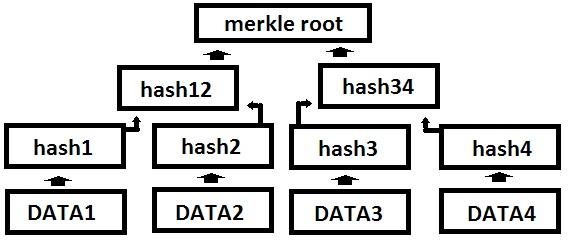
\includegraphics[width=8cm]{mroot.jpg}
\end{center}

Every transaction has a hash associated with it. In a block, all of the transaction hashes in the block are themselves hashed (sometimes several times - the exact process is complex), and the result is the Merkle root. In other words, the Merkle root is the hash of all the hashes of all the transactions in the block. The Merkle root is included in the block header. With this scheme, it is possible to securely verify that a transaction has
been accepted by the network (and get the number of confirmations) by downloading just the tiny block headers and Merkle tree - downloading the entire block chain is unnecessary. This feature is currently not used in Bitcoin, but it will be in the future.

Each node is particularly and primarily interested in transactions that concern the
accounts that are controlled by their operators, perhaps some watched accounts (such
as those of counterparties). It needs to verify that all the transactions preceding them
beginning with emission (mining) have been arithmetically correct and that no double
spending has been attempted. It may also verify random transactions as a means of
spot-checking the network.

\newpage

\section{Solution}
The solution is a simplified Bitcoin client that doesn't store all the transaction and the blockchain, only transactions that are relevant to the wallet are stored. Every other transaction is thrown away or simply never downloaded. The block chain is still used and broadcast transactions are still received, but those transactions are not and cannot be checked to ensure they are valid. This mode of operation is fast and lightweight enough to be run on a smartphone.


\subsection{Details}
Each balance is simply associated with an address and its public-private key pair. The money "belongs" to anyone who has the private key and can sign transactions with it. Moreover, those keys do not have to be registered anywhere in advance, as they are only used when required for a transaction. Each person can have many such addresses, each with its own balance, which makes it very difficult to know which person owns what amount. For instance, Bob can generate a new public-private key pair for each individual receiving transaction in order to protect his privacy. The Bitcoin software encourages this behavior by default.

When Bob someone starts to use this simplified wallet, he generates new public-private key pairs, so the wallet knows the creation time of all its keys. To keep track of its future transactions, block contents before this time don't have to be downloaded, only the headers, so it's much faster to bootstrap the system in this way. The method is similar to bitcoinj's fast catchup. This way you can sync with the chain just by downloading headers and some transactions and Merkle branches, but sometimes this is still too slow. 

It can further be augmented with bitcoinj's chekpoint files. These are generated using the BuildCheckpoints tool that can be found in the tools module of the bitcoinj source code. BuildCheckpoints downloads headers and writes out a subset of them to a file. That file can then be shipped with your application. When you create a new BlockStore object, you can use that file to initialize it to whichever checkpointed block comes just before your wallets fast catchup time (i.e. the birthday of the oldest key in your wallet). Then you only need to download headers from that point onwards.

Checkpoints are called checkpoints because, like the upstream Satoshi client, once you've initialized the block store with one bitcoinj will refuse to re-organise (process chain splits) past that point. In fact, it won't even recognize that a re-org has taken place because the earlier blocks don't exist in the block store, thus the alternative fork of the chain will be seen merely as a set of orphan blocks. For this reason the BuildCheckpoints tool won't add any checkpoints fresher than one month from when it's run - it only takes a few seconds to download the last months worth of chain headers, and no fork is likely to ever be longer than one month.

When a transaction is broadcast over the network we say it is pending inclusion in a block. Mining nodes will see the transaction, check it for themselves and if it's valid, include it in the current block they're trying to solve. Nodes do not relay invalid transactions. Your app will receive pending transactions, add them to the wallet, and run event listeners. 

\subsubsection{Bloom filtering}
By default the PeerGroup and Wallet will work together to calculate and upload Bloom filters to each connected peer. A Bloom filter is a compact, privacy preserving representation of the keys/addresses in a wallet. When one is passed to a remote peer, it changes its behavior. Instead of relaying all broadcast transactions and the full contents of blocks, it matches each transaction it sees against the filter. If the filter matches, that transaction is sent to your app, otherwise it's ignored. When a transaction is being sent to you because it's in a block, it comes with a Merkle branch that mathematically proves the transaction was included in that block. BitcoinJ checks the Merkle branch for each transaction, and rejects any attempts to defraud you.

Bloom filters can be noisy. A noisy filter is one that matches more keys or addresses than are actually in your wallet. Noise is intentional and serves to protect your wallet privacy - a remote node can't know if a matched transaction is really yours or not. In theory, wallet keys/addresses could be split up across each connected node for even more privacy. Essentially it's a bandwidth vs privacy tradeoff - a higher FP rate confuses remote eavesdroppers more, but you have to download more useless data as a result.

% Mivel mi DHT-t használunk, ezért Bloom filtert használni arra, hogy a sajátjaidon kívül más tranzakciót is eltárolj nem lehetséges, mivel a DHT elég jól meghatározza, hogy pontosan milyen ranzakciókat tárolj el. Egy ilyen Bloom filter esetén a többi node nem tudná hogy kinél keressen egy adott tranzakciót, mindenkit végig kéne kérdezni. arra viszont, hogy a saját tranzakcióinkat eltároljuk hasznos lehet, mert gondolom gyorsabb ezzel ellenőrizni mondjuk egy blokk kihirdetésénél hogy benne van-e a mienk. viszont adhat false pozitívta, de ez sem baj, mert akkor eltárolunk még pluszba néhány random tranzakciót, ez nem fogja befolyásolni a rendszer működését.

\subsection{Something}

Nodes operating this way can form a system that stores each transaction of the network and doesn't rely on other nodes to verify the integrity of transactions they are interested in.

Each node stores transactions that concern the accounts that are controlled by their operators. Furthermore, they store some other transaction, so an eavsdropper won't be able to decide which transaction (public key) belongs to the node. If there's a sufficiently large number of simplified nodes in the network, they will be able to store every bitcoin transaction. If a node needs some information on a specific transaction, it will send a request to the node that stores this transaction, and that node will reply with the requested information.

The main question is how to distribute the transactions among the nodes in a way they can easily find which node stores which transactions.
The solution is based on distributed hash tables. 

A distributed hash table (DHT) is a class of a decentralized distributed system that provides a lookup service similar to a hash table; (key, value) pairs are stored in a DHT, and any participating node can efficiently retrieve the value associated with a given key. Responsibility for maintaining the mapping from keys to values is distributed among the nodes, in such a way that a change in the set of participants causes a minimal amount of disruption. This allows a DHT to scale to extremely large numbers of nodes and to handle continual node arrivals, departures, and failures. DHT forms an infrastructure that can be used to form peer-to-peer content distribution.

In this network the hash of a transaction will play the role of the key, and the raw transaction will be the value. When there's a new transaction, each node forwards it through the network until it reaches the node responsible for it. That node then stores the transaction. Another node can retrieve this transaction by sending a request message with the hash of the transaction. This message is forwarded by the other nodes, until it reaches the node that stores the transaction. This node will reply with the raw transaction.

% itt azt nem tudom, hogy ha egy node-nek kell egy raw tranzakció, akkor azt mi alapján tudja lekérni. pl lehet h a hashét pont nem tudja, csak más adatokat róla... na most itt lehetséges-e nem hash alapján keresni? hát sztem nem nagyon... bár egy node-ot nyilván az ő tranzakciói érdeklik, amiről tud minden adatot, csak azt nem hogy benne van-emár egy blokkban. ez esetben csak emiatt akar körbeérdeklődni a tranzakcióról, és ekkor tudja ezt a hash-el csinálni. de más esetekben nem tudom hogy kéne 

We need to define how to partition the keyspace and find a proper routing protocol.


\subsection{Key space partitioning}

We need to map the hash of transactions to some node id.

Nodes identify themselves and find another nodes by their IP addresses. They store the IP addresses of nodes they previously connected to in their local peers.dat file. So the simplest way is to use IP addresses as node ids in the keyspace partitioning.

A transaction hash is a 32 bytes hexadecimal number, we need to map them to IP addresses. An easy way is to calculate the SHA256 hash of the IP addresses, and the node with the closest hash value to the transaction hash will store the transaction.

We treat the keys (hash of IP adresses) as points on a circle and define the distance of two keys as the distance traveling clockwise on the circle from one key to the other. So the circular keyspace is cut inti contiguous segments whose end points are the hash of node ids (IP addresses). If $id_1$ and $id_2$ are two adjacent node ids, with a shorter clocwise distan from $id_1$ to $id_2$ then $id_1$ will store all the values between $id_1$ and $id_2$. (Like in the chord DHT.)

Since values of a hash function are uniformly distributed, node ids will be uniformly distributed in the keyspace. It implies that nodes will have to store the about same amount of transactions.

 %itt a következő a problémám: ha valaki megfigyeli egy node forgalmát (h milyen tranzakciókat tárol el) akkor mivel nem csak a sajátját tárolja el nem tudja h mik az ő tranzakciói. de a tarnzakciók azonosítójából ki tudja szűrni h azt a node azért tárolta-e el mert közel van az id-jéhez vagy mert az övé a tranzakció. erre ugye megoldás lenne h a node nem hozza nyilvánosságra az id-jét, de ekkor a későbbiekben leírt routingot nem lehetne megvalósítani... vagy persze egymás között eltitkosítva küldözgetnek üzenetet, gondolom ez amúgy is így van, de... hát szóval ez megint csak problémákat vet fel





\subsection{Routing protocol}

A suitable routing protocol is necessary for forwarding and requesting transactions and adding and deleting nodes.

A node can send messages to nodes whose IP address is known to it (stored in its local peers.dat). For these nodes it can calculate their id (hash of IP address).

If a new node is added to the network,  it first finds some nodes already in the system.
% Ki kell írni hogy hogyan találhat ilyet: ugyanúgy mint egy normál bitcoin esetén
The new node sends its id  (in this chapter i refer as id to to the hash of IP addresses) to these nodes. These nodes will find in their peer.dat database the node which id is closest to this node's id in the sense of the aboved defined distance (they hash the stored IP addresses and check it), and forward the message to it. If this node can find another node closer to this new node it will forward this message, and so on until the message reaches the node closest to the new node. This node won't find anyone closer to the new node, so it won't forward the message.

This node halves its key space (so half of the transactions that were previously stored by this node will be stored by the new node) and sends a message to the new node with its id, half of its transactions and the range of transaction hashes it should store later; furthermore it stores this new node as its children. The new node will store this node as its father

Example: $id_1$ and $id_2$ are two adjacent nodes, and $id_3$ is a newly arrived node such that $id_3$ is between $id_1$ and $id_2$. In this case a message will reach $id_1$ with the new nodes id. $id_1$ know cheks that its closer to it than to $id_2$. It sends its own is ($id_1$) to $id_3$ along with $id_2$ and trhe transactions between $id_3$ and $id_2$ (they were stored by $id_1$ but from now on they will be stored by $id_3$). From $id_2$ $id_3$ will know that the transactions it should store range from $id_3$ to $id_2$.
%és még a mögötte lévő node id-ja

This way the new node will know which transactions it should store in the future and will store some other transaction in its database. Furthermore it knows its two neighbours, so if a routing message arrives to it the node will be able to decide which way to forward it.

This new node will also store the id of the nodes it sent the first message to. This way the node will know nodes further to it, not only its neighbours. This will fasten up a routing. And in the future if it gets a message from a new node, itt will store its id as well.

If a node leaves the system, it notifies its father node and its children. It sends the children the id of its father node, and the children will store it as their new father. It sends a message to the father with all its stored transactions and the children ids. The father will redistribute the transactions among its children.

% itt csak két gyereke között kell megosztani a tranzakcicót, akik közvetlenül a kilépő node előtt és után voltak

A routing protocol: assume that node A wants to find a transaction. It sends a request message with the transaction hash to the node in its peer.dat file whose id is closest to the transaction hash. This node will forward this transaction hash with the id of the original node to the node in its peer.dat file with the closest id to the hash and so on, until it reaches the node who actually stores that transaction. This node will send a the transaction to the original node and stores this node's id.

Basically, if a node gets a message from a node previously unknown to it it will store its id.

When broadcasting a transaction a node stores the ones that belong to him or that are close to him. When broadcasting a block each node stores the block header and checks the transactions in it and stores merkel branches of the previously stored transactions. Since nodes stores all the block headers, with the merkel branch they can verify a transaction.

%szerintem ha mindenki eltárolja az összes block header-t és az összes tranzakció valahol a networkben el van mentve, akkor ezzel tudnak verifikálni mindent, és megvalósul a decentralizáltság. ellenvetéseket várok.. :)


\subsection{}
First step: the DHT method works only if there's a sufficiently large network of these simplified clients. Until that time the clients will work as follows: from the creation of the wallet they check every broadcast message wheter it contains a transaction they are interested in. If there's no such transaction, they drop the message. After a transaction they're interested in is broadcasted, they start to check the generated blocks wheter it cointains that transaction or not. With this method they can verify a transaction. If a transaction is stored in a block the simplified wallet stores the corresponding Merkel branch.

Nodes can store some other transactions as well so that attackers won't know which transactions belong to them.

Nos ide jöhet egy kis számítgatás arról, hogy hány ilyen lightweight kiliens esetén válthatunk át a fent leírt rendszerre. A számítás menete a következő lenne: ha jól számolom a hash értéke összesen $2^{128}-1$-féle lehet. Mi azt szeretnénk hogy egy kliens ne tároljon aránytalanul sok infót a többiekhez képest. A uniform distr. miatt mindenki kb a tranzakciók $n$-edrészét tárolja, ha $n$ kliens van. Tegyük fel hogy akkor van baj ha valaki mondjuk egy y hosszú szakaszról tárol minden infót (ennél rövidebb szakaszról még gond nélkül eltárolja, de ez már túl sok). Akkor annak a vsz-e hogy egy kliens enyi infót tárol az megeygezik annak a vsz-ével, hogy az ő hash-e felvesz egy értéket és az utána következő y értéket más kliens hash-e nem veszi fel:

$$\mathbb{P}(\text{y hosszú szakaszról tárol egy kliens})=\left(\frac{2^{128}-1-y}{2^{128}-1}\right)^{n-1}$$

Ha meg tudjuk határozni y értékét, akkor tetszőleges valószínűség mellé meg lehet mondani, hogy milyen nagy n-nél érdemes átállni erre a DHT-s dologra. Ehhez tudni kéne hogy mondjuk egy smartphone-os bitcoin-os alkalmazásnál kb mennyi adatot tárolhatna el az alkalmazás a telefonon. Az eltárolt adatok a block header-ekből és a tranzakciókból állnak. Az eddigi összes blockheader méretét ha megkeressük plusz hogy mekkora egy tranzakció, akkor abból tudni fogjuk hogy hány tranzakciót tárolhat egy client hozávetőlegesen. A tárolható tranzakciók számából meghatározható y (a számolásnál a saját tranzakciók tárolását tekinthetjük sztem elhanyagolható méretűnek, mert az egész hálózat méretéhez képest valóban elhanyagolható. de itt tehetünk fel egyéb dolgokat is a saját tranzakciók méretéről, pl valahogy átlagolhatnánk-nem tudom hogy- és egy konstans értéket rendelünk hozzá). Ha megvan y, akkor lehet kijelentéseket tenni n-re, grafikonokat rajzolni, ilyenek.

Úgyhogy ehhez jó lenne valami számszerű adatokat találni.

%Nos ezt nem tudom h mennyire működik így jól, de lényegében a bitcoinj is ezt csinálja, szóval szerintem elfogadható

\subsection{}
Further problems: avoid double spending, attacks, level of trust in other nodes

%ezeket a dolgokat át kéne gondolni, hogy miért nem lehetséges duoble spend, milyen támadások lehetnek, blablabla... 



\newpage
\begin{thebibliography}{9}
\bibitem{}
https://en.bitcoin.it/wiki/Main\_Page
\label{bitcoinwiki}

\bibitem{}
http://en.wikipedia.org/wiki/Distributed\_hash\_table
\label{dhtwiki}

\bibitem{}
https://code.google.com/p/bitcoinj/
\label{bitcoinj}

\end{thebibliography}

\end{document}